
\section{Numerical Experiments}

\begin{figure}[ht]
  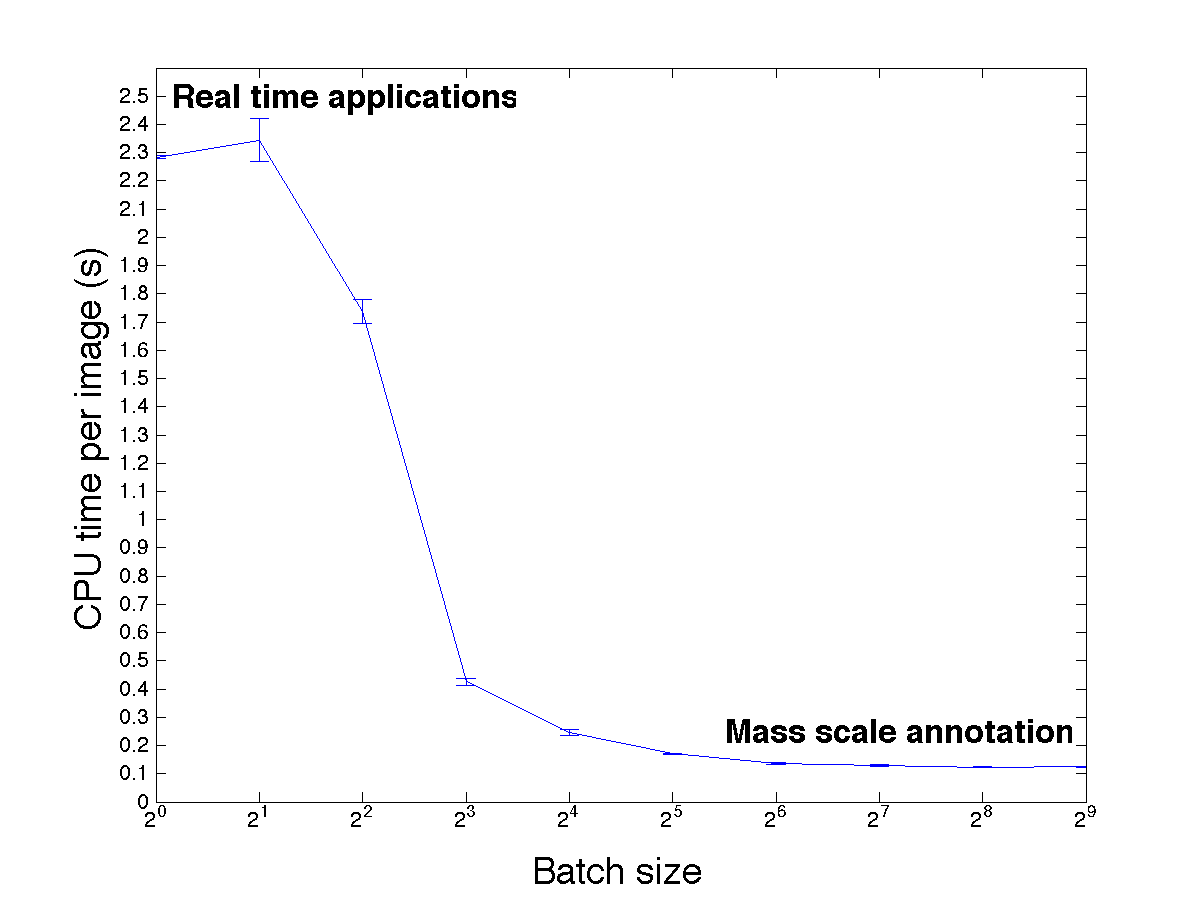
\includegraphics[width=0.48\textwidth]{img/eval_per_batch.png}
  \caption{CPU computational time per image for various batch sizes.}
\end{figure}
\begin{figure}[ht]
  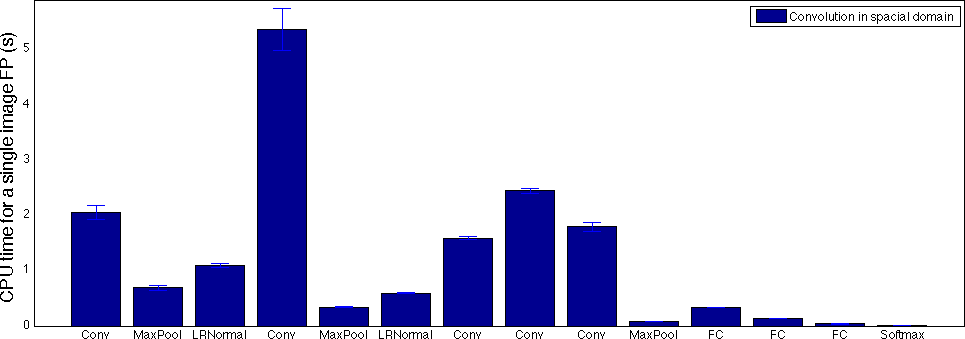
\includegraphics[width=0.48\textwidth]{img/eval_per_layer_per_batch_128_batch_size.png}
  \caption{Per layer breakdown of execution time for mini batch of size 128. Such size of mini batch gives optimal per image CPU time.}
\end{figure}
\begin{figure}[ht]
  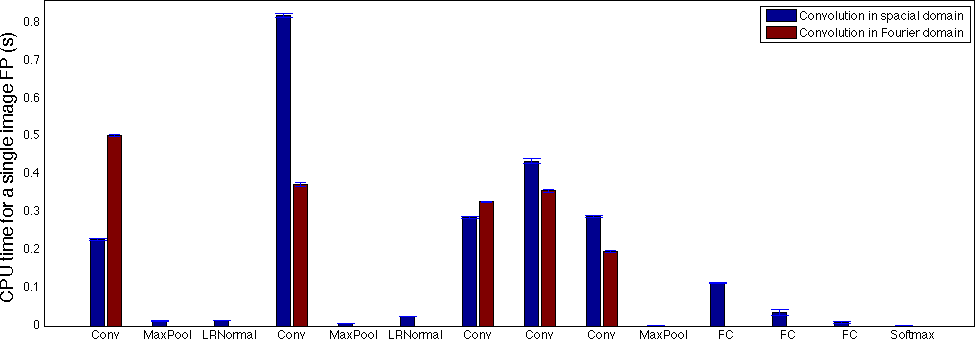
\includegraphics[width=0.48\textwidth]{img/eval_per_layer_per_batch_1_batch_size.png}
  \caption{Per layer breakdown of execution for mini batch of size 1. Use for real time applications.}
\end{figure}


\begin{figure}[ht]
  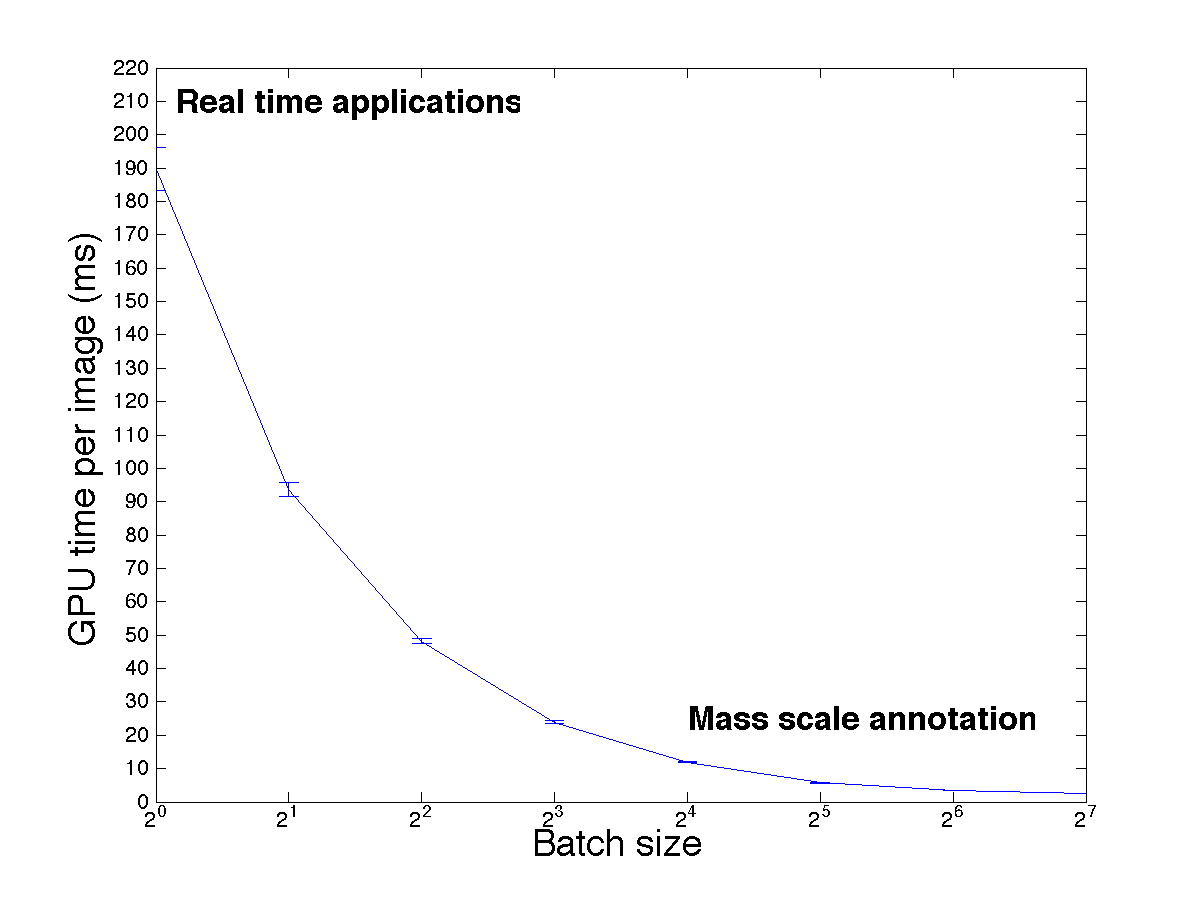
\includegraphics[width=0.48\textwidth]{img/eval_per_batch_GPU.png}
  \caption{GPU computational time per image for various batch sizes.}
\end{figure}
\begin{figure}[ht]
  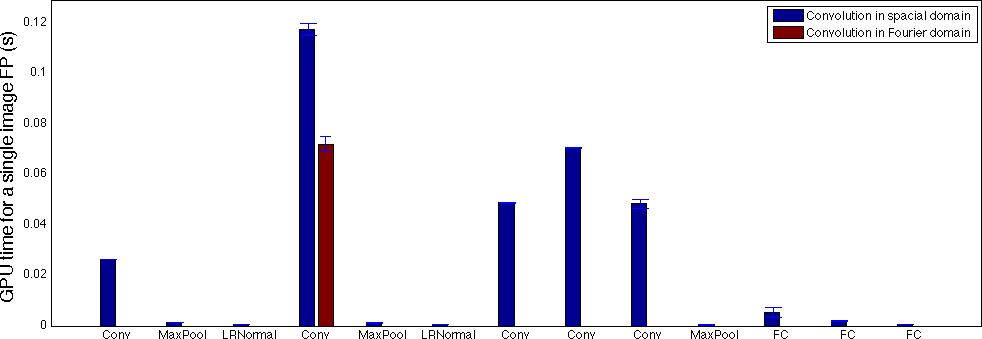
\includegraphics[width=0.48\textwidth]{img/eval_per_layer_per_batch_GPU_128_batch_size.png}
  \caption{Per layer breakdown of execution time for mini batch of size 128. Such size of mini batch gives optimal per image GPU time.}
\end{figure}

\subsection{Testing time}

on GPU: Michael can help.

on CPU

\subsubsection{Monochromatic}

\subsubsection{Linear combination of filters}

\subsubsection{Separable filters}


\subsection{ Denoising}
\begin{figure}[ht]
  \begin{minipage}[b]{0.48\linewidth}
  	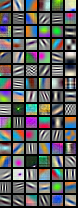
\includegraphics[width=\textwidth]{img/first.png}
  \end{minipage}
  \begin{minipage}[b]{0.48\linewidth}
  	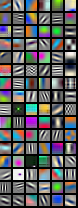
\includegraphics[width=\textwidth]{img/first_appr.png}
  \end{minipage}
  \caption{(Left) Original filters, (Right) approximated filters. (this pictures are too big, and should contain white separation).}
\end{figure}
